\documentclass[12pt,a4paper,twoside,titlepage,openright,headsepline,listof=totoc,index=totoc,chapterprefix,bibliography=totoc]{scrreprt}


\newif\ifpdfhere
\ifx\pdfoutput\undefined
\pdfherefalse % we are not running pdflatex
\else
\pdfoutput=1 % we are running pdflatex
\pdfcompresslevel=9     % compression level for text and image;
\pdfminorversion=6
\pdfheretrue
\fi

\ifpdfhere
%\usepackage{techreport}

\usepackage[pdftex,bookmarks=true,bookmarksopen=false,bookmarksnumbered=true,linktocpage,colorlinks=true,backref,pagebackref, linkcolor=blue,  citecolor=blue, urlcolor=blue]{hyperref}
%% Weitere Hyperrefeinstellungen
\hypersetup{%
pdfauthor={Markus von Detten, Stephan Hildebrandt, Christian Heinzemann, Marie Christin Platenius, Jan Rieke, Julian Suck, Dietrich Travkin}
,pdftitle={Story Diagrams -- Syntax and Semantics}
,pdfsubject={Technical Report}
%% fuer die Screen-Version: blue
,linkcolor=blue,anchorcolor=blue,citecolor=blue,filecolor=blue,menucolor=blue,urlcolor=blue
% fuer die Print-Version: black
% ,linkcolor=black,anchorcolor=black,citecolor=black,filecolor=black,menucolor=black,pagecolor=black,urlcolor=black%
}

\usepackage[pdftex]{graphicx}
\usepackage{thumbpdf}

\graphicspath{{figures/}}

\fi


% *** amsfonts ***
% Paket  : amsfonts
% Zweck  : f"ur spezielle Mathematik-Schriftarten (z.B. geschwungenes NP)
% Hinweis: Die Symbole erh"alt man mit \mathcal{NP}
% Doku   : Dokumentation zu finden unter (SuSE-Linux 7.0):
%          /usr/share/doc/packages/te_latex/texmf/fonts/amsfonts/amsfndoc.dvi
\usepackage{amsfonts}
\usepackage{algorithmic}
\usepackage{listings}
\lstset{ % 
basicstyle=\footnotesize,
tabsize=3,
language=[Visual]C++,
backgroundcolor=\color{white}
}
\usepackage{url}
\usepackage{color}
\usepackage{tabularx}
\usepackage[normalem]{ulem}
\usepackage[T1]{fontenc}
\usepackage{inputenc}

\usepackage{std_authorlist}

% *** amsmath ***
% Paket  : amsmath
% Zweck  : f"ur spezielle Mathematik-Symbole (z.B. nat"urliche und reelle Zahlen)
% Hinweis: Die Symbole erh"alt man mit \mathbb{N}
% Doku   : Dokumentation zu finden unter (SuSE-Linux 7.0):
%          /usr/share/doc/packages/te_latex/texmf/latex/amsmath/amsldoc.dvi
\usepackage{bbm}

\usepackage{amsmath}
\usepackage{amssymb}
\usepackage{ntheorem}
\usepackage{mathtools}

% *** fancyvrb ***
% Paket  : fancyvrb
% Zweck  : f"ur das Einf"ugen von Quellcode
% Doku   : Dokumentation zu finden unter (SuSE-Linux 7.0):
%          /usr/share/doc/packages/te_latex/texmf/latex/fancyvrb/fancyvrb.ps
\usepackage{fancyvrb}

% *** floatflt ***
% Paket  : floatflt
% Zweck  : f"ur Textfluss um Abbildungen und Tabellen
% Doku   : Dokumentation zu finden unter (SuSE-Linux 7.0):
%          /usr/share/doc/packages/te_latex/texmf/latex/floatflt/floatflt.dvi
\usepackage{floatflt} 

% *** graphics ***
% Paket  : graphicx
% Zweck  : zum Einbinden von EPS-Graphiken
% Doku   : Dokumentation zu finden unter (SuSE-Linux 7.0):
%          /usr/share/doc/packages/te_latex/texmf/latex/graphics/grfguide.ps
\usepackage{graphicx}

% \DeclareGraphicsExtensions{.png,.jpg}
% *** ngerman ***
% Paket  : ngerman
% Zweck  : f"ur Umlaute, deutsche Silbentrennung usw.
% Hinweis: ngerman benutzt im Gegensatz zu german die neue Rechtschreibung
%          (wichtig f"ur die Silbentrennung)
% Doku   : Dokumentation zu finden unter (SuSE-Linux 7.0):
%          /usr/share/doc/packages/te_latex/texmf/generic/styles/gerdoc.dvi
%\usepackage{ngerman}
%\selectlanguage{english} % Dokumentensprache auf deutsch stellen
%\usepackage[english]{babel}

% *** times ***
% Paket: Times
% Zweck: Schrift Times benutzen (sieht wesentlich besser als die Standardschrift aus)
\usepackage{times}
\usepackage[rightcaption]{sidecap}

%\usepackage{setspace}

\addtolength{\oddsidemargin}{1.5cm}
\addtolength{\evensidemargin}{-1.5cm}
%\addtolength{\topmargin}{-0,2cm}
%\addtolength{\textheight}{+1.5cm}
%\addtolength{\textwidth}{-0cm}

\sloppy
\usepackage{supertabular} 

%% snake-oil f�r den Satz
 \pretolerance=100           %% Textsatz: interner Parameter zur Steuerung des Zeilenumbruchs \tolerance 300              %% 1414 Bewertungsgrenzwert f�r schlecht umbrochene Zeilen
 \hfuzz=0.2pt                %% Grenze, ab der eine overfull hbox gemeldet wird
 \vfuzz=0.2pt                %% Grenzwert, ab dem die �berf�llung einer \vbox protokolliert wird
 \hbadness 1414              %% Grenzwert f�r �schlechte� Zeilen, bzw. Boxen
 \vbadness	1000              %% Grenzwert f�r eine �schlechte� \vbox 
 \emergencystretch 1em       %% zus�tzlicher dynamischer Leerraum
 \hyphenpenalty=30           %% Strafpunkte bei Silbentrennung �ber Absatz hinweg
 \widowpenalty=100000          %% falls letzte Zeile auf neue Seite gebrochen wird.
 \clubpenalty=100000           %% wenn erste Zeile eines Absatzes auf alter Seite bleibt.
 \doublehyphendemerits=50    %% Aufeinanderfolgende Silbentrennungen eher vermeiden. 

\setcounter{secnumdepth}{3}

%use this command to denote figure element that appear inside a figure
\newcommand{\fe}[1]{\textsf{\small #1}}

\theoremstyle{break}
\newtheorem{definition}{Definition}[section] 
\newtheorem{bsp}{Beispiel}[section] 

\usepackage{fancyhdr}

\pagestyle{fancy} 
\fancyhf{} 
\fancyhead[EL,OR]{\thepage} 
\fancyhead[ER]{\small\MakeUppercase{\leftmark}}
\fancyhead[OL]{\small\MakeUppercase{\rightmark}}

%% \TODO{}-Command um schnell zu sehen was noch zu machen ist ;)

\RequirePackage{xspace}
\providecommand{\fuj}[1][\xspace]{{\scshape FUJABA}#1}


\setlength{\marginparwidth}{2cm}

%\usepackage[colorinlistoftodos, textwidth=2.0cm, disable]{todonotes}
\usepackage[colorinlistoftodos, textwidth=2.0cm]{todonotes}
\newcommand{\todoall}[1]{\todo[inline, color=green!40]{Alle: #1}}
\newcommand{\todoch}[1]{\todo[inline, color=yellow!40]{Chris: #1}}
\newcommand{\todomvd}[1]{\todo[inline, color=cyan!40]{Markus: #1}}
\newcommand{\tododt}[1]{\todo[inline, color=blue!40]{Dietrich: #1}}
\newcommand{\todoib}[1]{\todo[inline, color=pink!30]{Ingo: #1}}
\newcommand{\todojr}[1]{\todo[inline, color=orange!30]{Jan: #1}}



\begin{document}                     % und los!

	% ************************************************************
	% *****                    Titelseite                    *****
	% ************************************************************

	\setcounter{page}{1}
	\pagenumbering{Roman}

	\begin{titlepage}
	\thispagestyle{empty}
	{\center

			\vspace{1.5cm}
            {\LARGE  {\bf Story Diagrams -- Syntax and Semantics}}
			\\
			\vspace{2cm}
			{\Large Technical report} \\
			\vspace{1,25cm}
			 
			
			Markus von Detten, Christian Heinzemann, Marie Christin Platenius, \\
			Jan Rieke, Julian Suck, and Dietrich Travkin \\
			Software Engineering Group\\			
			Heinz Nixdorf Institute\\
			University of Paderborn\\
			Zukunftsmeile 1\\
			D-33102 Paderborn, Germany\\
			$[$t.b.a.$]$@mail.uni-paderborn.de\
			\\ \ \\
      		\ \\    		
      		
            \vspace{1cm}
            
			Stephan Hildebrandt\\
			Department System Analysis and Modeling\\
			Hasso-Plattner-Institut\\
			Prof.-Dr.-Helmert-Str. 2-3\\
			D-14482 Potsdam, Germany\\
			stephan.hildebrandt@hpi.uni-potsdam.de\\
            
            \vspace{2,5cm}
            
            Version: 0.1
			
			\vspace{2,5cm}
			Paderborn, \today



		}
	\end{titlepage}


	
%
%	 ~
%	\newpage
	
%	\input{content/eid.tex}
        
%	\newpage
%	~
% 	

% 	
% 	\newpage
% 	~	
	
	\tableofcontents
	\cleardoublepage
% 	~
% 
% 	\newpage
% 	~

% 	\newpage

	\pagenumbering{arabic}
	\setcounter{page}{1}
	%\setstretch{1.2}
	% ------------------------------------------------------------------ Seminarausarbeitung -----------------------------------------------------------------
	\chapter{Introduction (Jan)}
% Problem Area
To tackle the complexity of modern technical systems, the engineering of such systems is heavily based on models.
Models are considered first-class artifacts of the development.
They describe different parts of the system in development, from different viewpoints and on different abstraction levels.
For instance, models are used to describe the structure and behavior of a software system, improving the overall comprehensibility of the system.
These models can then be employed to automatically generate code, reducing the risks of implementation errors.

As models evolve during the development process and different models have to be translated into each other and kept consistent, model transformations are a crucial part such a development process.
Model transformations are used to define in which way models can be changed, e.g., to specify refactoring operations.

Furthermore, model transformations itself can be employed to precisely specify the behavior of a system at run-time.
If, for example, a system should react to environment changes by reconfiguration, these reconfigurations can be described by model transformations which define how to reconfigure the system.
They furthermore allow a formal analysis, e.g., to prove that certain properties still hold after applying a transformation.

Story diagrams~\cite{ZSW99,FNTZ00,Zun01} are a powerful visual formalism for specifying model transformation, based on the well-known concept of graph transformation systems.
They feature declarative parts to specify object patterns which are matched and altered in the source model and combine them with an imperative part to specify the control flow of the transformation execution.
The concrete syntax of story diagrams extends the concrete syntax of UML activity diagrams.

% Problem
Since their introduction in 1998, several extensions to story diagrams have been proposed.
Furthermore, some semantic issues have been identified in the original concept~\cite{TMG06}.
In addition, the main story diagram tool, the Fujaba tool suite, has undergone major redesigns the last years; these redesigns also affected the story diagram implementation.
Moreover, new approaches like the Story Diagram Interpreter have emerged.

% Approach
In this technical report, we seek to provide a complete reference of the syntax and semantics of story diagrams.
It consolidates previous publications in a single document.
We provide definitions for the abstract and the concrete syntax as well as the semantics of story diagrams.

%Evaluation
As an example, we show how story diagrams can be used to specify refactoring operations on structural software models like class diagrams.

% Structure
\todojr{Struktur}

\section*{Old stuff from rejected paper}
% Problem Area
In model-driven software engineering, model transformations play a central role in transforming models of higher abstraction levels into more concrete models. 
Such transformations are written in special purpose languages which offer explicit support for common transformation tasks like matching elements of the source model.
While the development of current model transformation languages focused on those model transformation specific tasks, classical issues like inheritance and structuring were neglected.
As a result, the transformations are often concise and efficient but hardly maintainable.

% Problem
Story diagrams~\cite{ZSW99,FNTZ00,Zun01} form a special model transformation language.
They feature declarative parts to specify object patterns which are matched and altered in the source model and combine them with an imperative part to specify the control flow of the transformation execution.
The concrete syntax of story diagrams extends the concrete syntax of UML activity diagrams.
A specific challenge for story diagrams is the missing support for the invocation of other story diagrams.
We require these invocations to account for aspects like the increased complexity of binding parameters and result values in a graphical language as well as dynamic dispatching of calls.

% Related Work
Some of the related transformation languages like ATL, QVT Operational, or Henshin already offer some support for structuring transformations into sub transformations.
However, no existing hybrid and graphical transformation languages addresses all of the aforementioned challenges. 

% Approach
In this paper, we present an approach to tackle the lacking feature of invoking story diagrams.
Our solution supports binding the parameter values as well as the result values of the invoked diagram.
We also introduce polymorphic dispatching in our solution, i.e., the invoked diagram is chosen at run-time based on the actual types of the bound parameter values.
Consequently, the story diagram meta-model as well as the existing interpreter for story diagrams \cite{GHS09} have to be extended to support the new concepts. 

% Validation
We show the effectiveness of our approach in a qualitative study of an existing transformation implemented in story diagrams. In the study, we estimate the potential to reduce the total amount and size of the story diagrams in our initial implementation. The results show a significant improvement in transformation size, leading to reduced complexity and thus an increase in the long-term maintainability of the transformation.

% Contribution summary
 

	\chapter{Foundations}
\label{sec:foundations}

\todoall{What else do we need to address in this chapter?}

\section{Graphs and Graph Transformations}
\label{sec:foundations:simpleGTS}

Graphs consist of nodes and edges where an edge always connects two nodes. Nodes are used to represent objects and edges denote relationships between these objects. In course of this document, we will assume edges to be directed, i.e., they have a source node and a target node. In the most simple case, neither nodes nor edges have a predefined semantics \cite{Roz97}.

\begin{figure}[htbp]
  \centering
  
\includegraphics[scale=1.5]{figures/SimpleGraph}
  \caption{Simple Graph}
  \label{fig:simpleGraph}
\end{figure}

Figure \ref{fig:simpleGraph} shows an example of a simple graph with three nodes and four edges. The nodes are visualized a circles, the edges are visualized as arrows. An edge may have the same node as a source and target node. Such an edge is called a \emph{self-edge}.

\emph{Graph transformation rules} specify allowed modifications of graphs. They consist of a left-hand side (LHS), a right-hand side (RHS), and a so-called rule morphism. Both, the LHS and the RHS are graphs while the rule morphism specifies which nodes of the LHS and RHS are considered to be the same. This information is required for the application of a graph transformation rule to a graph.

\begin{figure}[htbp]
  \centering
  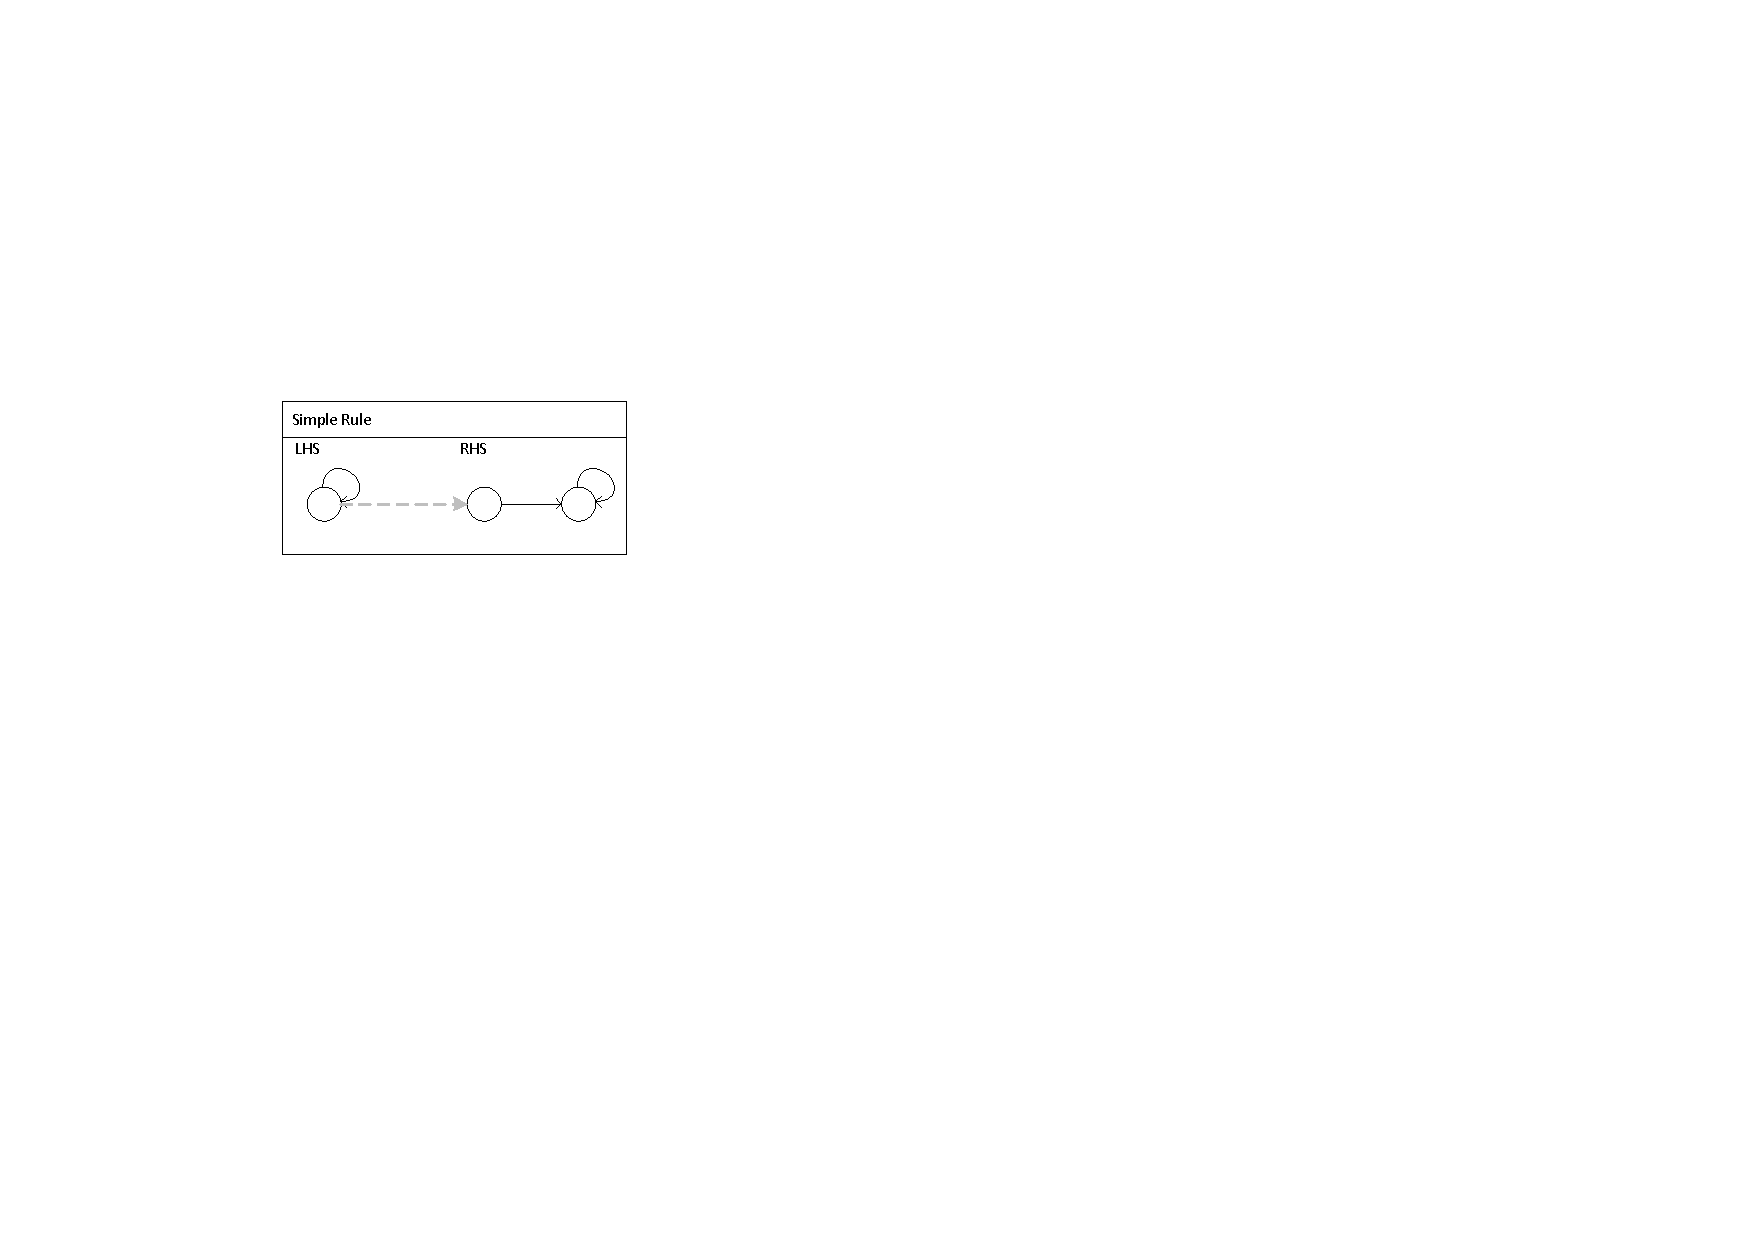
\includegraphics[scale=1.5]{figures/SimpleGTRule}
  \caption{Simple Graph Transformation Rule}
  \label{fig:simpleGTRule}
\end{figure}

Figure \ref{fig:simpleGTRule} shows an example of a graph transformation rule. The LHS contains only node node with a self-edge. The RHS contains two nodes connected by an edge where the right node of the RHS has a self-edge as well. The rule morphism is visualized by the grey, dotted arrow. It specifies that the node of the LHS and the left node of the RHS are considered to be the same.

The application of a graph transformation rule to a graph is called a \emph{graph transformation} \cite{EEPT06}. The graph on which the rule is to be applied is called the \emph{host graph}.
The application of a graph transformation rule to a graph is performed in three steps. In the first step, an occurrence of the LHS of the graph transformation rule in the host graph is searched. Such an occurrence is called a \emph{match} of the graph transformation rule. If a match has been found, all nodes and edges that occur in the LHS but not in the RHS are deleted from the host graph. In this step, the rule morphism is used to decide which nodes do not occur in the RHS. In the third step, all nodes and edges that occur in the RHS but not in the LHS are added to the host graph. After the application of the graph transformation rule, there exists a match of the RHS into the host graph.

\begin{figure}[htbp]
  \centering
  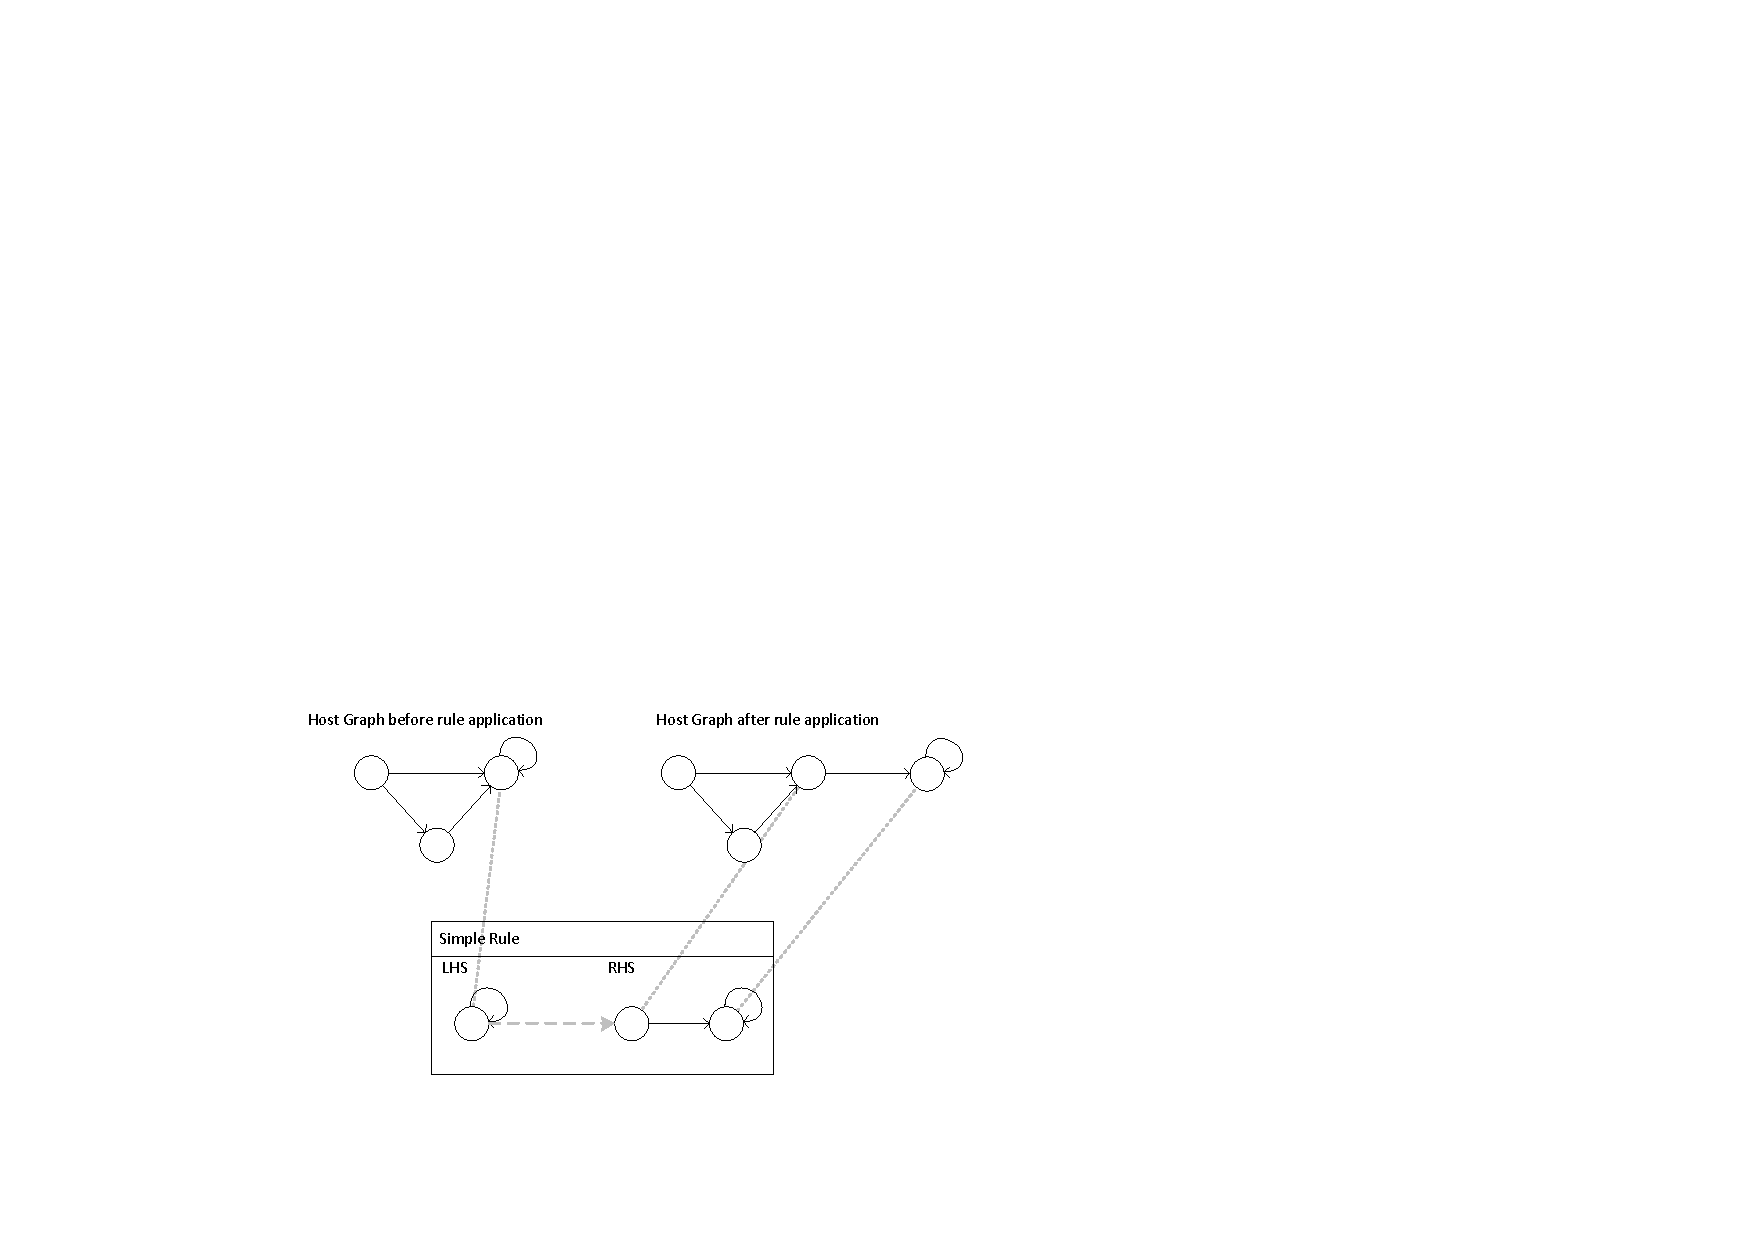
\includegraphics[width=\linewidth]{figures/GTApplication}
  \caption{Application of a Graph Transformation Rule}
  \label{fig:GTApplication}
\end{figure}

Figure \ref{fig:GTApplication} shows an example of a graph transformation that applies the graph transformation rule of Figure \ref{fig:simpleGTRule} to the graph of Figure \ref{fig:simpleGraph}. The matching of the LHS into the host graph is visualized by a gray, dotted line. Then, the graph transformation rule deletes the self-edge from this node. Afterwards, a new node with a self-edge is created and connected to the previously matched node by an edge. The match of the RHS into the host graph after the rule application is again shown by gray, dotted lines.

In the field of algebraic graph transformations, the two most popular approaches for applying a graph transformation rule to a graph are the
\emph{double-pushout approach} \cite{Roz97} and the \emph{single-pushout
approach} \cite{Roz97}. The definition of story diagrams follows the
single-pushout approach. Besides the more theoretical differences the two
approaches differ in the handling of two special situations that might occur
upon rule application.

The first situation is the following. Assume the left-hand side of a rule
consists of two nodes. The first node is to be deleted and the second one is
to be preserved. Both of these nodes may be matched to the same node in the host
graph. In this situation, it is not clear if the node in the host graph is to be
deleted or preserved. The double-pushout approach explicitly forbids the application of the rule in such
situations. The single-pushout approach allows such situations and gives
deletion priority over preservation.

The second situation deals with dangling edges. It occurs if a certain node is
to be deleted but some of its incident edges are to be preserved. The
transformation would lead to a non-valid graph in which the edges would not have
either a source or a target node. The double pushout approach does not allow
such situations and instead requires that incident edges are explicitly
deleted. The single-pushout approach allows such situations and implicitly
deletes edges if one of the source or target nodes are deleted.

In general, matches of graph transformation rules are homomorphisms of the LHS of the rule to the host graph. That allows to match two nodes of the LHS to the same node of the host graph leading to first situation mentioned above. Such situations may be prevented by using isomorphisms for matching the LHS. Then, each node of the LHS must be matched to a unique node of the host graph. Thus, using isomorphic matchings solves the first situation when using single pushouts.

\section{Typed Attributed Graph Transformations}
\label{sec:foundations:typedAttrGTS}

Graphs and according graph transformations as introduced in Section \ref{sec:foundations:simpleGTS} are a very basic approach to modeling behavior. When using graph transformations for modeling behavior for object-oriented software or as a foundation for defining the semantics of modeling languages, it is necessary to distinguish different types of nodes and edges in a graph in order to give them semantics. 

Therefore, story diagrams are based on typed attributed graph transformations \cite{EEPT06}. Typed attributed graph transformations introduce a type graph and node attributes. The type graph defines different types of nodes and edges and it defines which types of edges are allowed for which type of nodes. Additionally, nodes may carry attributes like, e.g., objects in an object-oriented programming language. Accordingly, the type graph specifies inheritance relations between types of objects which are also known from object oriented programming languages.

\section{Type Model used in this Report}

\begin{figure}[htbp]
  \centering
  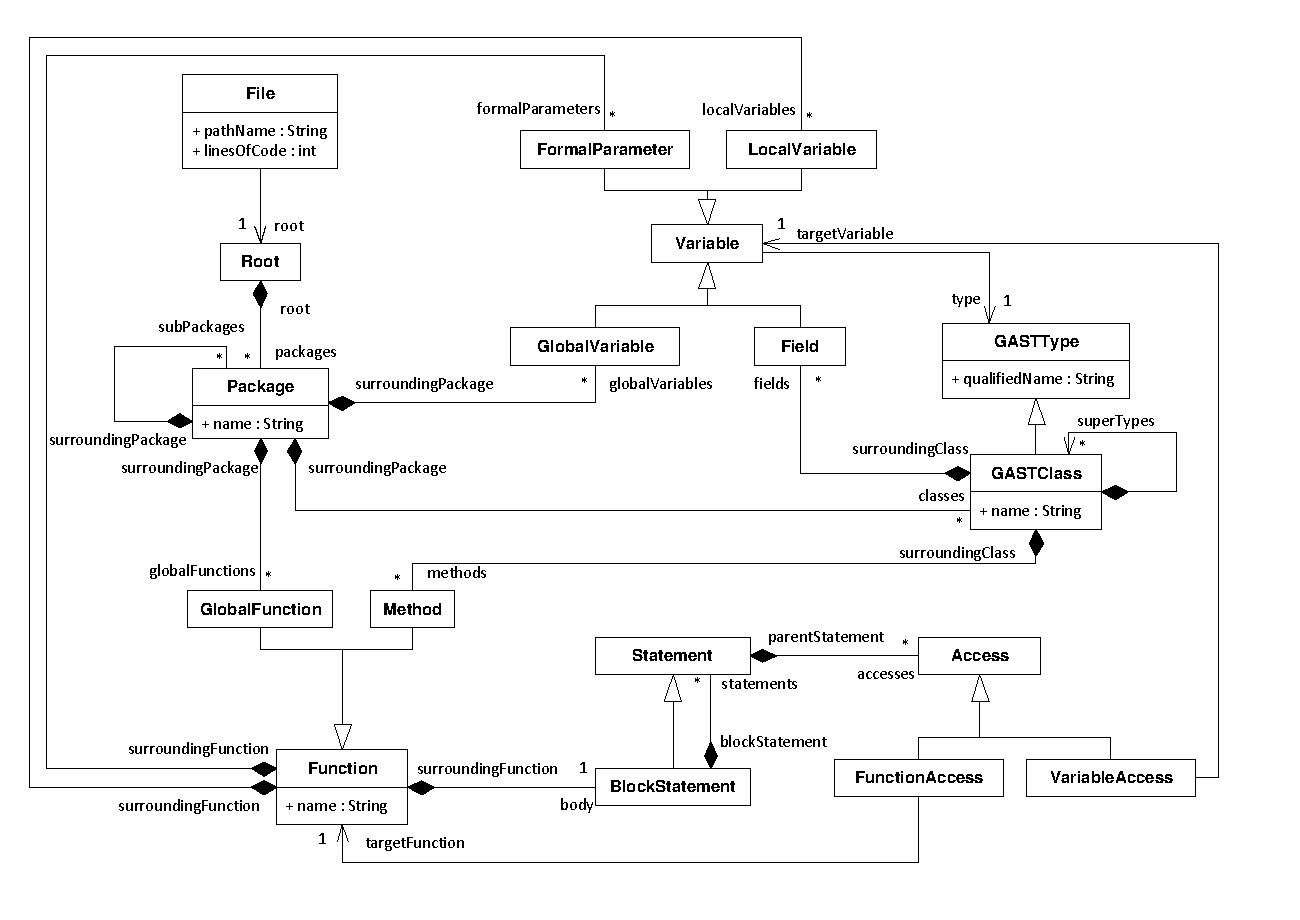
\includegraphics[width=\linewidth]{figures/gast-mm}
  \caption{Type model of a generalized abstract syntax tree (GAST).}
  \label{fig:gast-mm}
\end{figure}

The type model used in the examples in this report describes the structure of an abstract syntax tree. In particular it is an updated and slightly simplified version of the generalized abstract syntax tree (GAST) meta model developed in the QBench project \cite{QBench}. The GAST was developed to provide a unified syntax tree model for different programming languages like Java, C, and C++.
Figure~\ref{fig:gast-mm} shows an excerpt of that meta model. Especially some specialized sub classes have been omitted for clarity reasons.

\begin{description}
\item[Root] The \fe{Root} element is the central element of every GAST model. All other elements are reachable from the \fe{Root} node via composition relations.
\item[File] Elements of the GAST, e.g., classes and packages, can be assigned to files in the file system. A \fe{File} element holds references to those classes and packages and a String containing the path to the file.
\item[Package] Similar to packages in Java, the \fe{Package} element provides name spaces and visibilities. A \fe{Package} element can contain other packages, classes, global variables, and functions.
\item[GASTType] The \fe{GASTType} element represents data types like primitive data types and classes. The attribute \fe{qualifiedName} contains the unique, fully qualified name of the type.
\item[GASTClass] Classes are represented by the element \fe{GASTClass} in the GAST and are a sub type of the \fe{GASTType}. A \fe{GASTClass} holds references to its methods, attributes, and inner classes. A \fe{GASTClass} can be assigned to a \fe{Package}.
\item[Function] \fe{Function} is the super type for all executable operations. In addition to a name attribute, a \fe{Function} can have a number of local variables and formal parameters. The return type of a \fe{Function} is determined by its \fe{DeclarationTypeAccess}, a sub class of \fe{Access} (not shown in Figure~\ref{fig:gast-mm}). A \fe{Function} always contains a block statement which, in turn, can contain other statements.
\item[GlobalFunction] A \fe{GlobalFunction} element represents a globally accessible operation, i.e., an operation that does not belong to a class. They can be assigned to a name space defined by a package. For example, C functions are represented by \fe{GlobalFunctions}.
\item[Method] Functions that belong to an class are represented by \fe{Method} elements, a sub type of \fe{Function}.
\item[Variable] \fe{Variable} is a super type for all kinds of variables. A \fe{Variable} always has a name and a type.
\item[LocalVariable] \fe{LocalVariables} are variables that are contained in a \fe{Function}.
\item[FormalParameter] \fe{FormalParameters} are variables that represent the parameters of a \fe{Function},
\item[GlobalVariable] \fe{GlobalVariables} are variables that are globally accessible within a given scope. The scope is determined by the package in which the \fe{GlobalVariable} is contained.
\item[Field] The \fe{Field} element represents class variables. Therefore it is contained in a \fe{GASTClass}.
\item[Statement] A \fe{Function} consists of a number of \fe{Statements}. There are multiple sub classes of \fe{Statement} which represent the different kinds of statements. Most of them are omitted here. A \fe{Statement} can contain a number of \fe{Accesses}.
\item[BlockStatement] The \fe{BlockStatement} is a special kind of statement which can contain other \fe{Statements}. It is the root element of all \fe{Statements} contained within a \fe{Function}.
\item[Access] An \fe{Access} represents the use of a \fe{Variable} or a \fe{Function}. It always belongs to a certain \fe{Statement}.
\item[FunctionAccess] A \fe{FunctionAccess} represents the use of a \fe{Function} in a \fe{Statement} and therefore references the accessed \fe{Funtion} element.
\item[VariableAccess] A \fe{VariableAccess} represents the use of a \fe{Variable} in a \fe{Statement} and therefore references the accessed \fe{Variable} element.
\end{description}


	\chapter{Concepts} \label{sec:Concepts}

\todoall{Description of elements should follow this structure: What is it for? What does it do? Examples in concrete syntax + explanation}

\section*{Old stuff from rejected paper}
In this section, we will briefly introduce story diagrams and their current features. 
Story diagrams combine
UML activity diagrams and graph transformations by embedding graph replacement rules into the activities.
This allows the activities in Figure \ref{fig:transformationOverview} to be specified formally by graph replacements while preserving the general control flow structure of the example transformation.

In terms of the classification of model transformations proposed by Czarnecki and Helsen~\cite{Czarnecki06}, story diagrams are an endogenous, in-place transformation language.
It has both declarative (pattern matching) and operational elements (specification of control flow):
Its control flow allows a deterministic selection of the graph replacement rules to be applied, with a (non-deterministic) pattern matching in the graph replacement rules.
It can also be used for inter-model transformations to create a new target model from a given source model, as seen in the example given in this paper. 
In order to execute story diagrams, code generation \cite{GBD07} and interpretation \cite{GHS09} are supported.

In the following, we will describe the graph transformations, the so-called story patterns, in Section~\ref{sec:StoryPatterns}.
Afterwards, we will explain how control flow can be modeled by using elements from activity diagrams in Section~\ref{sec:StoryDiagrams}.

	\section{Story Patterns} \label{sec:StoryPatterns}

Story patterns describe graph replacement rules that can be embedded into the activities of a story diagram. They are based on labeled, attributed graphs that are extended by a type model \cite{FNTZ00}. 
The types and references that are specified in the type model are used to type the nodes and edges within the story pattern.
Type models for story diagrams can be created, e.g., by using EMF Ecore \cite{SBP+08}.
In our example, we will use the meta-models shown in Figures~\ref{fig:sourceMetamodel} and~\ref{fig:targetMetamodel} as type models. The type model supports inheritance and polymorphism, i.e., a node of type \fe{Classifier} matches objects of types \fe{Classifier}, \fe{Class}, and \fe{PrimitiveType}.
This allows specifying graph replacement rules for object-oriented models.

In order to provide a concise notation, story patterns apply a short-hand notation depicting left-hand side and right-hand side in one graph. Nodes and edges being created (or deleted) are annotated with \small \verb|<<create>>| \normalsize (or  {\small \verb|<<destroy>>|\normalsize}, respectively). The matching of story patterns in a host graph requires an isomorphic matching of the pattern's left-hand side in the host graph, i.e., two nodes of the pattern may not be matched to the same node in the host graph \cite{FNTZ00,Roz97}. The matching is performed with respect to the types of the type model. The deletion of nodes is applied according to the Single Pushout Approach (SPO, \cite{Roz97}), i.e., dangling edges resulting from the deletion of nodes are deleted as well.

Figure~\ref{fig:SP} shows an example of a story pattern that simply adds a class to the set of classifiers of the source system (cf. Figure~\ref{fig:sourceMetamodel}).

\begin{figure}[htbp]
\begin{center}
  
\includegraphics[width=0.25\textwidth]{figures/StoryPattern}
  \caption{Simple story pattern}
  \label{fig:SP}
\end{center}
\end{figure} 
	
	\section{Story Diagrams} \label{sec:StoryDiagrams}

\subsection*{Old stuff from rejected paper}
Story diagrams are an extension of UML 1.4 activity diagrams \cite{UML} that embed story patterns into the activities.
That allows to model basic control flow structures like branches or loops.
Figure \ref{fig:controlFlow} shows a story diagram that embeds the story pattern of Figure \ref{fig:SP} into one of its activities.
The purpose of the story diagram is to create a new class in the source system if no class with the name given by the parameter \fe{className} already exists. 

\begin{figure}[tbp]
\begin{center}
  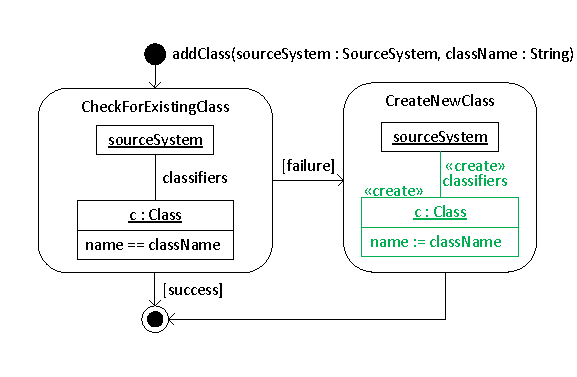
\includegraphics[width=0.7\textwidth]{figures/ControlFlow}
  \caption{Control flow in story diagrams}
  \label{fig:controlFlow}
\end{center}
\end{figure}

In the first activity, the embedded story pattern tries to bind a class with the respective name in the source system. The \fe{sourceSystem} is given as a parameter to the story diagram and can be used as a \emph{bound} node by referring to the name of the parameter. A bound node is signified in the concrete syntax by omitting its type information. Then, the story pattern tries to bind an object of type \fe{Class} to the \emph{unbound} node named \fe{c} such that the attribute condition is fulfilled. 
If this pattern can be matched successfully, i.e., the class already exists, the activity is left via the \fe{[success]} transition and the story diagram terminates.
If no such class can be found, the matching fails and the activity is left via the \fe{[failure]} transition.
Then, the second activity creates the class, links it to the source system, and sets the respective name. 
Additionally, it is possible to add boolean conditions and an \fe{[else]} to the transitions to model more specific conditions.

In general, an initial matching is established by the parameters. This matching is extended by the story patterns in the activities. Then, the matching is propagated to the next activity along the transitions. If a story pattern fails, the current matching is not changed. In subsequent activities, an object previously bound to a node \emph{c} can be referenced using a bound node with name \emph{c}.

The specification of the transformation outlined in Figure~\ref{fig:transformationOverview} can only be accomplished by specifying loops because it requires iterating over all classifiers of the system and all methods of the classes. Loops can be modeled using \emph{forEach activities}.
The story patterns in forEach activities are matched as long as new matchings can be found.
They are visualized by a double border line as depicted in Figure~\ref{fig:forEach}. The transformation formalizes the informal description of Figure~\ref{fig:transformationOverview} using the current features of story diagrams.

\begin{figure}[htb]
\begin{center}
  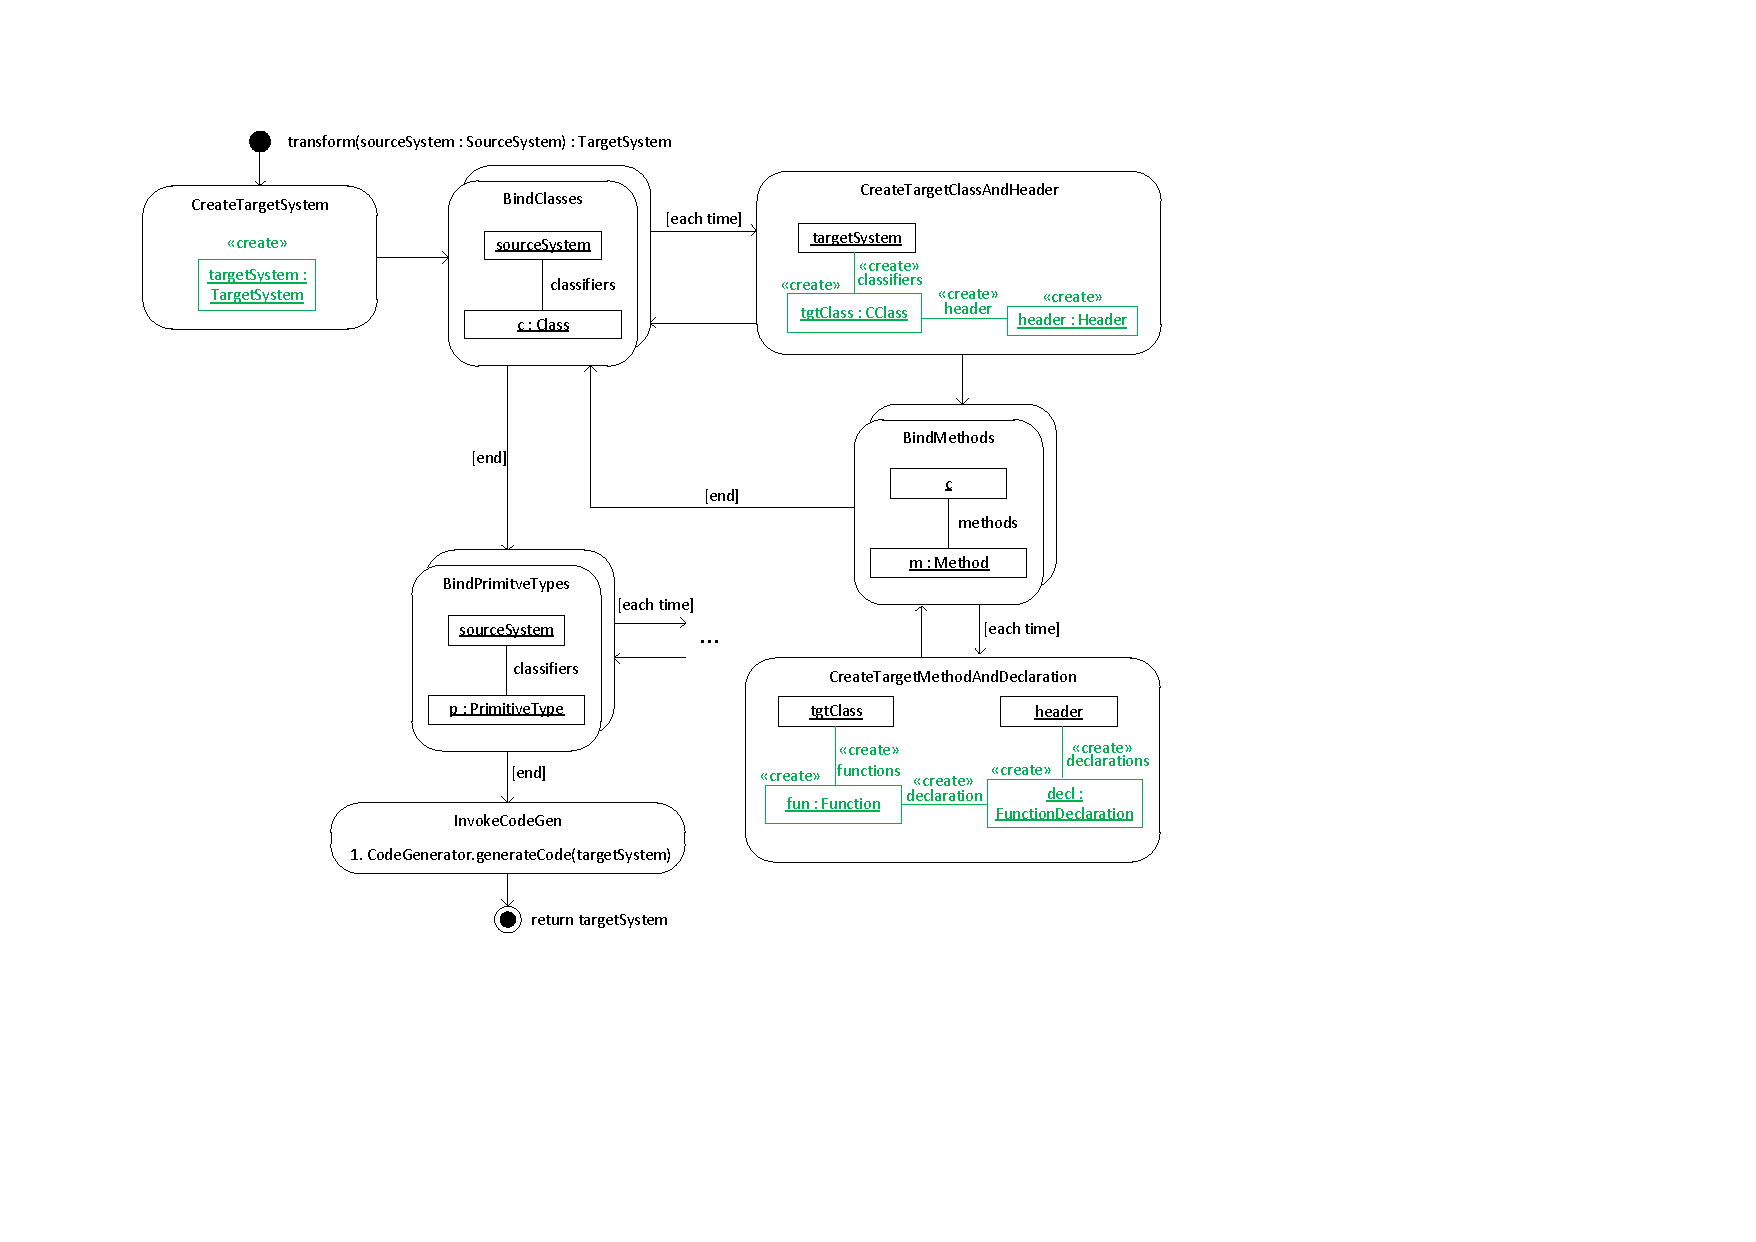
\includegraphics[width=\textwidth]{figures/ForEach}
  \caption{Example of a complex transformation including several forEach activities}
  \label{fig:forEach}
\end{center}
\end{figure}

The story diagram creates a target system in its first activity. Then, all classes of the source system \fe{sourceSystem} are matched. For each match that has been found, the forEach activity is left via the \fe{[each time]} transition. Then, the third activity creates a respective class and its header in the target system. Afterwards, all methods of the class \fe{c} of the source system are matched. Again, the forEach activity is left for each new match using the \fe{[each time]} transition. After all methods have been transformed, the control flow returns to the activity \fe{Bind classes} to bind the next class. It is required that a control flow that has left a forEach activity eventually returns to this activity to obtain a correct story diagram.

After transforming the classes, all primitive types of the source model have to be transformed. We omit the details here due to space limitations. 
Finally, the target system object \fe{targetSystem} is returned by the story diagram as indicated by the annotation \fe{return targetSystem} on the stop node.

Hitherto, story diagrams only support proprietary calls to library functions called collaboration statements. In Figure \ref{fig:forEach}, the activity \fe{InvokeCodeGen} contains such a call to the code generator. The call only is a string expression that does neither allow type checking of the input parameters nor getting a matching of return values, i.e., the return values cannot be used in the story diagram.

\subsection{Applications of Stroy Diagrams (Dietrich)}
2 worlds: with and without methods\ldots

\subsection{General composition of Story Diagrams}
\begin{itemize}
  \item Based on UML 1.5 activity diagrams
  \item Grammar for story diagrams (based on grammar in diploma thesis of Thomas Klein (1999))
\end{itemize}

\subsection{Calls}

\todomvd{Wie sehen Calls (Method/Activity) aus?}

	\section{Expressions} \label{sec:Expressions}
	
	\section{Templates (Dietrich)}
	
 
	
	\chapter{Complete Example}

To illustrate our concept, we use a language transformation scenario: Suppose we have a model representing the abstract syntax graph (ASG) of a program. The ASG is language-specific, of course. If we want to generate code from the ASG for a target language other than the language on which the given ASG is based, one option is to transform the ASG first.
One example of this would be a transformation from Java to C++.

\begin{figure}[ht]

\begin{minipage}[b]{0.42\linewidth}
	\centering
	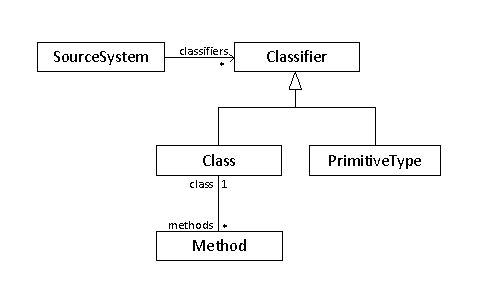
\includegraphics[scale=0.7]{figures/sourceMetamodel}
\caption{Source meta-model}
\label{fig:sourceMetamodel}
\end{minipage}
\hfill
\begin{minipage}[b]{0.55\linewidth}
\centering
	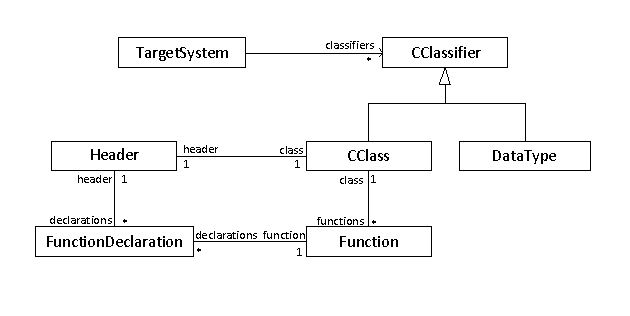
\includegraphics[scale=0.7]{figures/targetMetamodel}
\caption{Target meta-model}
\label{fig:targetMetamodel}
\end{minipage}

\end{figure}


Figure~\ref{fig:sourceMetamodel} shows a simplified meta-model for an ASG which acts as the source meta-model for our exemplary transformation scenario. A \fe{SourceSystem} consists of a number of \fe{Classifiers} which can either be \fe{PrimitiveTypes} or \fe{Classes}. Each \fe{Class} can have a number of \fe{Methods}.

The target meta-model for the transformation, shown in Figure~\ref{fig:targetMetamodel}, is slightly more complex.
The \fe{TargetSystem} consists of a number of \fe{CClassifiers} which are either \fe{DataTypes} or \fe{CClasses}.
An \fe{CClass} can contain a number of \fe{Functions}. In addition, each \fe{CClass} has a corresponding \fe{Header} which contains a \fe{FunctionDeclaration} for each \fe{Function} of the \fe{CClass}.


\begin{figure}[htbp]
\begin{center}
  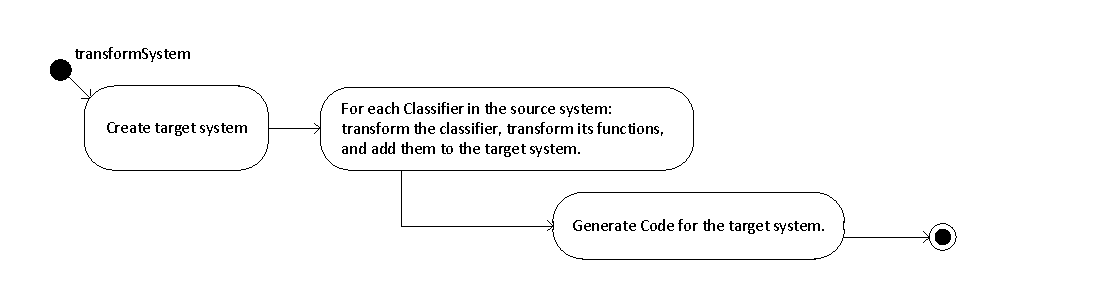
\includegraphics[width=\textwidth]{figures/transformationOverview}
  \caption{An activity diagram describing the example transformation}
  \label{fig:transformationOverview}
\end{center}
\end{figure}

Figure~\ref{fig:transformationOverview} shows an activity diagram which gives an overview of the transformation from a source ASG to a target ASG.
At first, the target system has to be created. Each classifier in the source system has to be transformed into a corresponding classifier in the target system. While primitive types can be transformed easily, headers have to be created for all transformed classes. For each method, a function has to be created and a corresponding function declaration has to be added to the correct header. In the end, the target system can be passed to the code generation mechanism.

\subsection{Requirement}

Das Beispiel muss enthalten:
\begin{itemize}
  \item Komplexer Kontrollfluss (success und failure, forEach, exception und finally, boolean conditions), verschiedene Node Types (normal, forEach, start, stop, Junction)
  \item StatementNode und TextualExpression
  \item Negative Anwendungsbedingung und komplexe negative Anwendungsbedingung (Subpattern eines Story Pattern)
  \item Calls inkl. polymorphic dispatching
  \item Expressions (Attribute Assigments, Attributvergleich beim Matching, Constraint eines Story Pattern), LinkConstraints (z.B. neue Methode als letzte in die Liste einsortieren, neue Methode in alphabetischer Reihenfolge einsortieren)
  \item SetObjects und Constraints fuer diese
  \item Structured Nodes und Flow Stops
  \item Pattern Matching: Optional, Maybe bound, Optional create, Optional destroy?
  \item Maybe construct, um Isomorphietest fuer zwei gebundene Objekte zu deaktivieren
  \item Templates
\end{itemize}	
	
	\chapter{Related Work}

\section*{Old stuff from rejected paper}

Model transformation has become an important research topic during the last years.
Several concepts and tools with different scopes and applications have been proposed.

Several model transformation approaches exist which are similar to story diagrams.

Here, we focus on those solutions that have a reasonable documentation available.
For a more comprehensive overview of transformation approaches see, for example, \cite{Czarnecki06}.
Current transformation tools can, for instance, be found in \cite{TTC2010}.

\emph{Henshin}~\cite{henshin2} is a model transformation language for in-place transformations of EMF-based models.
It uses pattern-based rewrite rules (called ``transformation rules'') and control-flow-based operational semantics (called ``transformation units'') on top of it.
Transformation units can also be called by other transformation units, also including parameters.
Henshin, however, does not provide support for polymorphic dispatching.
\emph{MOLA}~\cite{mola} is an in-place model transformation language with graphical syntax similar to story diagrams.
Transformation rules may consist of multiple matching and modification patterns, and the control flow inside a transformation rule can be specified, with a focus on the loop construct.  
Furthermore, it also allows calling other transformations rules, but does not support polymorphic dispatching.

\emph{Groove}~\cite{Ren04a} \todoch{Passt die Referenz? Hab die einfach mal aus dem Aigaion gefischt.Markus.} is a graph transformation tool with a focus on analyzing graph transformation systems.
Its rules consist of single rewrite patterns.
For instance, given a rule set and a start graph, Groove can explore the graph state space and use this for model checking.
It also features so called ``control programs'', which allow the user to restrict which rules can be applied and in which order.
\emph{VIATRA}~\cite{viatra}, a textual language, uses abstract state machines to specify the control flow and graph transformation rules for elementary model manipulations.
It also addresses modularization by reusable patterns that are called from the graph transformation rules. 

Although most of the story-diagram-like transformation languages include means for specifying control flow (including calling other transformation units), none of them supports polymorphic dispatching.
(Note that in most cases polymorphic dispatching can be emulated using other means, but doing so would result in a more complex and less maintainable rule set.)

However, looking at other transformation language types, there are some approaches that support polymorphic dispatching. 
For instance, \emph{Xpand}~\cite{xpand}, a model-to-text transformation language based on templates, uses ``polymorphic template invocation'' where the most specialized template available is used.
However, it only supports single dispatch, i.e., only one parameter is used to determine the used template.   

Considering exogenous, inter-model transformations, \emph{QVT Operational}~\cite{QVT} is an operational language that also allows polymorphic dispatching by its \fe{disjuncts} keyword.
A QVT-O mapping operation can declare that a call to it should be dispatched to other mappings.
In this case, the invocation of that mapping operation results in the execution of the first mapping whose signature fits the concrete parameters and whose \fe{when} clause evaluates to \fe{true}.
This is a more powerful construct than our solution, as it not only allows dispatching based on the actual type, but arbitrary constraints.
However, there must be a base rule where all dispatching possibilities are listed;
in our solution, all signature-compatible transformations with the same name are automatically used in dispatching, allowing a better modularization as well as an easier extension of the rule set.      
Furthermore, QVT-O is a textual transformation language which may not be well-suited in many cases~\cite{Moo09}.

In declarative inter-model transformation languages like \emph{Triple Graph Grammars} (TGGs) \cite{Sch94}, the control flow cannot be defined explicitly.
Instead, the order of the rule application is implicitly defined by preconditions of the transformation rules.
However, when more than one rule has a fitting precondition, the rule to be applied is selected non-deterministically, dependent on the concrete transformation tool implementation, or by a given rule priority.
Klar et al. \cite{Klar07} proposed a rule generalization concept with a precedence for the most refined rules, a solution similar to polymorphic dispatching.
In \emph{QVT Relations}~\cite{QVT}, which is similar to TGGs, control flow may also be explicitly specified by using \fe{where} clauses.

The \emph{Atlas Transformation Language} (ATL)~\cite{ATL} is a hybrid inter-model transformation language, integrating declarative and operational aspects.
It is similar to QVT, but only has a textual representation of the transformation rules.


\begin{itemize}
 \item Evtl. Loesungen zu M2M Transformation Aufgabe aus dem Tool Transformation Contest 2010 fuer weiteres Related Work anschauen
 \item Xpand
\end{itemize}

\section{Brainstormed topics from first meeting}
\todomvd{Endogen/Exogen}
\todojr{Henshin, ATL, PROGRES, AGG, TGGs, QVT-O, QVT-R}
\todoch{SDDs, TSSDs}
\todoall{Komponenten-Storydiagramme}
	
	\chapter{Conclusions}

\section*{Old stuff from rejected paper}

The specification of control flow has always been an integral part of story diagrams.
However, story diagrams did not support structuring complex transformations into several independent story diagrams up to now. 
In this paper, we described an extension of the existing formalism for the control flow to allow the invocation of other story diagrams, including parameters and return values.
Furthermore, we introduced a concept to polymorphically dispatch a call to the story diagram which matches the actual run-time types of the bound parameters. 

By this means, story diagrams become more flexible and reusable and allow a better structuring of the rule set. 
In a qualitative evaluation, we have discussed that these new features can help to reduce the size of the rule set and increase its maintainability.

As future work, we plan to investigate whether and how the polymorphic dispatching can be extended, for example, to allow arbitrary dispatching conditions similar to QVT-O.
We also plan to evaluate the maintainability, conciseness, and understandability of our approach in comparison to other model transformation languages in an empirical study.

\section{Future Work on report}
\begin{itemize}
  \item Formalization
  \item Verification
\end{itemize}
	
	%\setstretch{1}
        
% -------------------------------------------------------------
% Literaturverzeichnis 
% -------------------------------------------------------------
	\addtocontents{toc}{}         % Zum Inhaltsverzeichnis muss eine Leerzeile zugef"ugt werden, weil
                        	      % sonst das Literaturverzeichnis falsch im Inhaltsverzeichnis erscheint.
	\bibliographystyle{alpha}

	\bibliography{SdmPaper}

% ------------------------------------------------------------
% Appendix
% ------------------------------------------------------------

\appendix
	\chapter{Technical Reference}\label{sec-reference}
	
	\todoch{Paste the generated stuff here.}	

% ------------------------------------------------------------
% Abbilungsverzeichnis
% ------------------------------------------------------------
	%\listoffigures


% -------------------------------------------------------------
% Tabellenverzeichnis 
% -------------------------------------------------------------
    %\listoftables
	

	% ************************************************************
	% *****                      Ende                        *****
	% ************************************************************

\end{document}
